\section{Model HWIND}

Model łamliwości drzew HWIND powstał w celu wyznaczania maksymalnej prędkości wiatru przy których drzewo ulegnie złamaniu lub wyrwaniu (dla lasów sztucznie zalesianych). Został on opracowany dla sosny zwyczajnej i świerku pospolitego.

\begin{figure}[!h]
	\center
	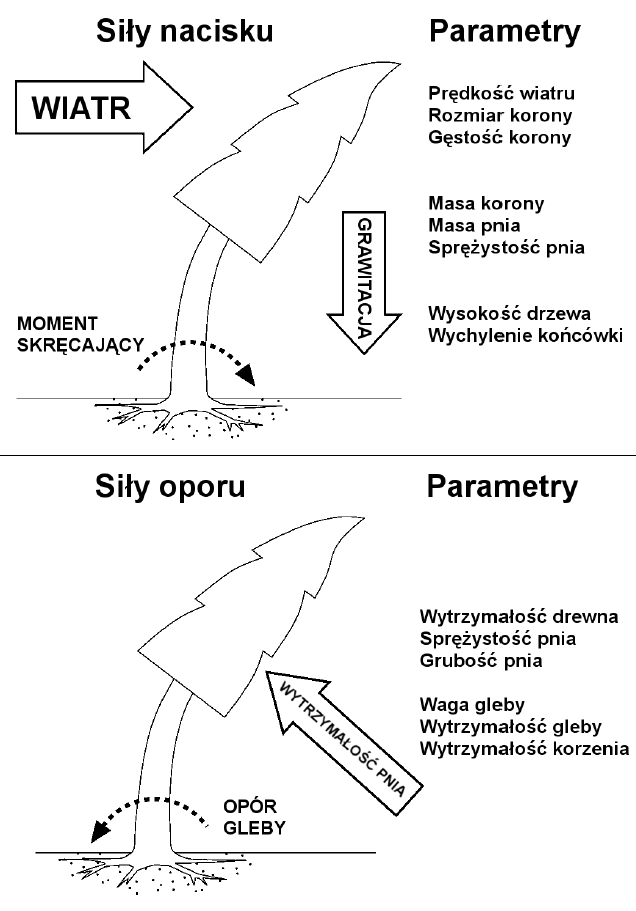
\includegraphics[scale=0.45]{HWIND1}
	\caption{Rozkład sił działających na drzewo dla modelu HWIND. Źródło: ~\cite{chm_mgza}.}
	\label{fig:HWIND1}
\end{figure} 

Rysunek ~\ref{fig:HWIND1} przedstawia siły działające na drzewo. Dokonany został podział na siły poziome i ~pionowe.
Pod naporem wiatru drzewo ugina się do momentu osiągnięcia punktu krytycznego, gdy siły nacisku (siła wiatru, siła grawitacji) zrównają się z ~siłami oporu (wytrzymałość pnia, wytrzymałość gleby wokół korzenia).

W celu wyznaczenia maksymalnego momentu skręcającego i ~granicznej prędkości wiatru przy której nastąpi zniszczenie drzewa, podzielone zostały one na 1~metrowe segmenty, dla których wyznaczone zostaną wartości sił.

Całkowita pozioma siła wiatru $F_w$ uzyskana zostaje poprzez sumowanie wartości siły wiatru obliczonej osobno dla każdego 1~metrowego segmentu ~\cite{chm_mgza}. Siła dla poszczególnego segmentu uzyskiwana jest ze wzoru:
\begin{equation}
\label{eq:windForce}
 F_w(z) = \frac{1}{2}C_d  \rho v_h^2 A(z)
\end{equation}
gdzie
\begin{description}
  \item[$C_d$] -- współczynnik tarcia
  \item[$\rho$ ]-- gęstość powietrza
  \item[$v_h$ ]-- prędkość pozioma dla danego segmentu
  \item[$A(z)$]-- przewidywana wielkość korony drzewa stawiająca opór wiatrowi
\end{description}

W celu uproszczenia obliczeń dokonana została aproksymacja powierzchni korony drzewa przez trójkąt równoramienny (świerk pospolity). Pole powierzchni pnia jest reprezentowane przez prostokąt. Model ten przedstawia rysunek \ref{fig:HWIND2}.

\begin{figure}[!h]
	\center
	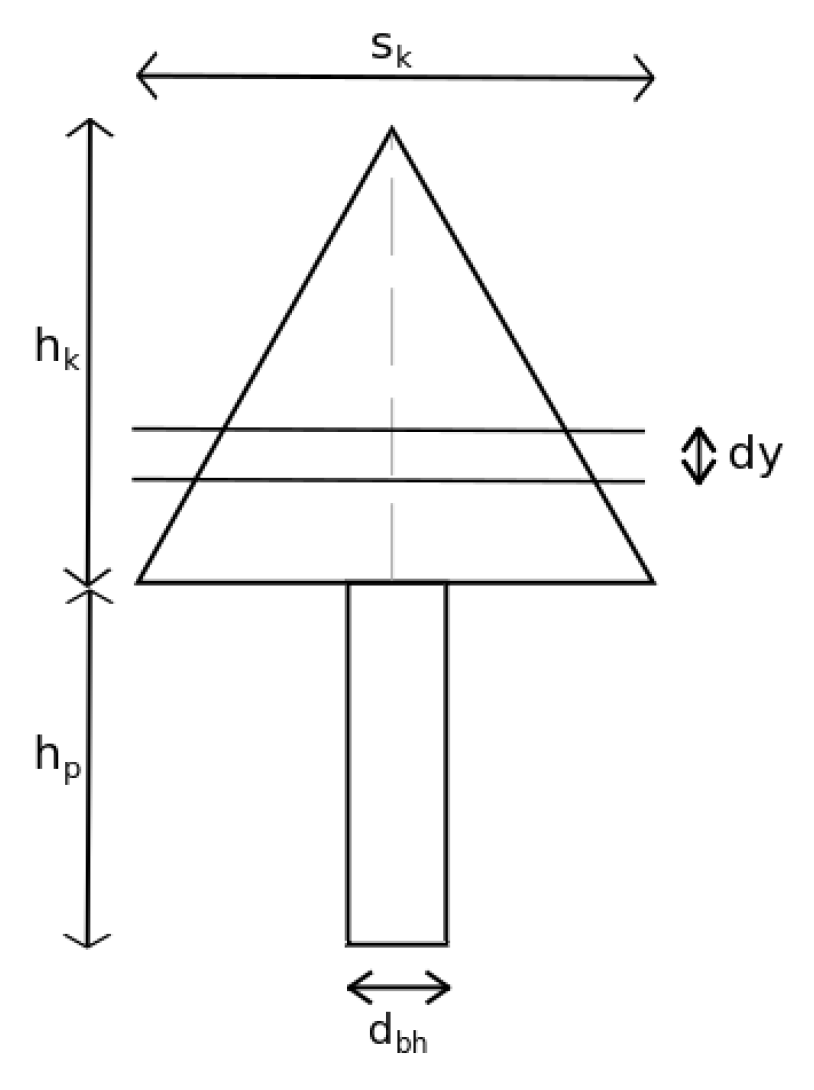
\includegraphics[scale=0.35]{HWIND2}
	\caption{Model powierzchni stawiającej opór wiatrowi. $s_k$ oznacza szerokość korony, $h_k$ -- wysokość korony, $h_p$ -- wysokość pnia, $d_{bh}$ -- średnicę pnia, $d_y$ -- wycinek powierzchni o wysokości 1m użyty przy w modelu HWIND. Źródło: ~\cite{chm_mgza}.}
	\label{fig:HWIND2}
\end{figure} 

W modelu należy uwzględnić fakt, iż pod wpływem wiatru powierzchnia korony ulega zmniejszeniu ~\cite{todo_jakies_zrodlo}. Redukcja powierzchni wynosi $20\%$ dla prędkości mniejszych od $11 \frac{m}{s}$, dla 
większych od $20\frac{m}{s}$ -- $60\%$. Dla wartości pomiędzy nimi współczynnik przepływu wiatru $S_t$ jest wyznaczany z następującego wzoru:
\begin{equation}
\label{eq:windFlow}
 S_t(z) = 0.044444v(z) - 0.28889
\end{equation}
gdzie
\begin{description}
  \item[$v(z)$] -- prędkość wiatru na wysokości z
\end{description}

Powierzchnia $A(z)$ wyznaczana jest przez jej iloczyn ze współczynnikiem $S_t$.
\\

Siła grawitacji wyznaczana jest dla każdego segmentu drzewa, a następnie sumowana. Wyznaczana jest ze wzoru:
\begin{equation}
\label{eq:gravityForce}
F_g(z) = m_c g
\end{equation}
gdzie
\begin{description}
  \item[$m_c$] -- masa korony drzewa
  \item[$g$] -- przyspieszenie ziemskie
\end{description}

Maksymalny moment skręcający drzewa $B_{max}(z)$ wyznaczamy dla każdego segmentu poprzez sumę siły wiatru $F_w(z)$ pomnożonej przez wysokość $\Delta z$, oraz siły grawitacji $F_g(z)$ pomnożonej przez odchylenie czubka drzewa od pionu $x(z)$ ~\cite{chm_ang}. Suma następnie zostaje pomnożona przez stosunek między maksymalnym, a średnim momentem ugięcia $f_{gust}$ oraz stosunek pomiędzy maksymalnym, a średnim współczynnikiem odległości pomiędzy drzewami $f_{gap}$. Zależność ta jest wyrażona następującym wzorem:

\begin{equation}
\label{eq:bendMoment}
B_{max}(z) = f_{gust} f_{gap} [ F_w(z) \Delta z + F_g(z) x(z)]
\end{equation}

Odchylenie czubka od pionu używane w powyższym wzorze ~(\ref{eq:bendMoment}) wyznaczane jest za pomocą wzoru ~\cite{chm_ang}:
\begin{equation}
\label{eq:crovnDeviation}
 x(z) =
\left\{
  \begin{array}{l r}
  	\frac{F_w a^2h(3- \frac{a}{h} - \frac{3l(z)}{h} }{6 \cdot MOE \cdot I} 	& \text{dla} \; z \leq a\\
    	\frac{F_w a^3 (2-\frac{3(l(z)-b)}{a} + \frac{(l(z) - b)^3}{a^3}}{6 \cdot MOE \cdot I} & \text{dla} \; z > a\\
  \end{array} \right.
\end{equation}
gdzie
\begin{description}
\item[$a$] -- wysokość środka korony
\item[$h$] -- wysokość drzewa
\item[$l(z)$] -- odległość od czubka drzewa na wysokości $z$
\item[$MOE$] -- współczynnik elastyczności drzewa
\item[$I$] -- powierzchniowy moment bezwładoności ($I = \pi \frac{d_{bh}^4}{64}$, gdzie $d_{bh}$ to średnica drzewa na wysokości $1.3m$
\item[$b$] -- odległość między czubkiem drzewa, a środkiem korony
\end{description}





